\documentclass[12pt,a4paper]{article}
% \usepackage[portuges]{babel}
% \usepackage[utf8]{inputenc}
% \usepackage[T1]{fontenc}
\usepackage{graphicx}

\usepackage{float}
\usepackage{enumerate}
\usepackage{makeidx}
\usepackage{booktabs}
\usepackage{pdfpages}
\usepackage{a4wide}
\usepackage{marvosym}

\setlength\oddsidemargin{0.3in}
\setlength\evensidemargin{-0.3in}
\setlength\headsep{15pt}
\setlength\footskip{30pt}

\usepackage{fontspec}
\defaultfontfeatures{Mapping=tex-text}
\setmainfont[
  Extension=.ttf,
  Path=font/,
  Scale=1.00,
  BoldFont={NewsGotTMed Regular},
  ItalicFont={NewsGoth Lt BT Light},
  ItalicFeatures={FakeSlant},
  AutoFakeSlant=0.3,
  BoldItalicFeatures=FakeSlant, 
]{NewsGotT Regular Fixed}

%Line Spacing
\usepackage{xspace}
\usepackage{setspace}
\onehalfspacing

% Language definitions
\usepackage{polyglossia}
\setmainlanguage{portuges}


% environment created for organization purposes, only.
\newenvironment{TODO}{%

  \color{blue} \itshape \begin{itemize}
}{%
  \end{itemize}
}


%---------------------------------------

% our addimage command
\newcommand{\addimg}[1]{%
  \begin{center}
    \includegraphics[width=0.75\textwidth]{#1}
  \end{center}
}

\newcommand{\RowStretch}[1]{\renewcommand{\arraystretch}{#1}}



%----------------------------------------------------------

\begin{document}

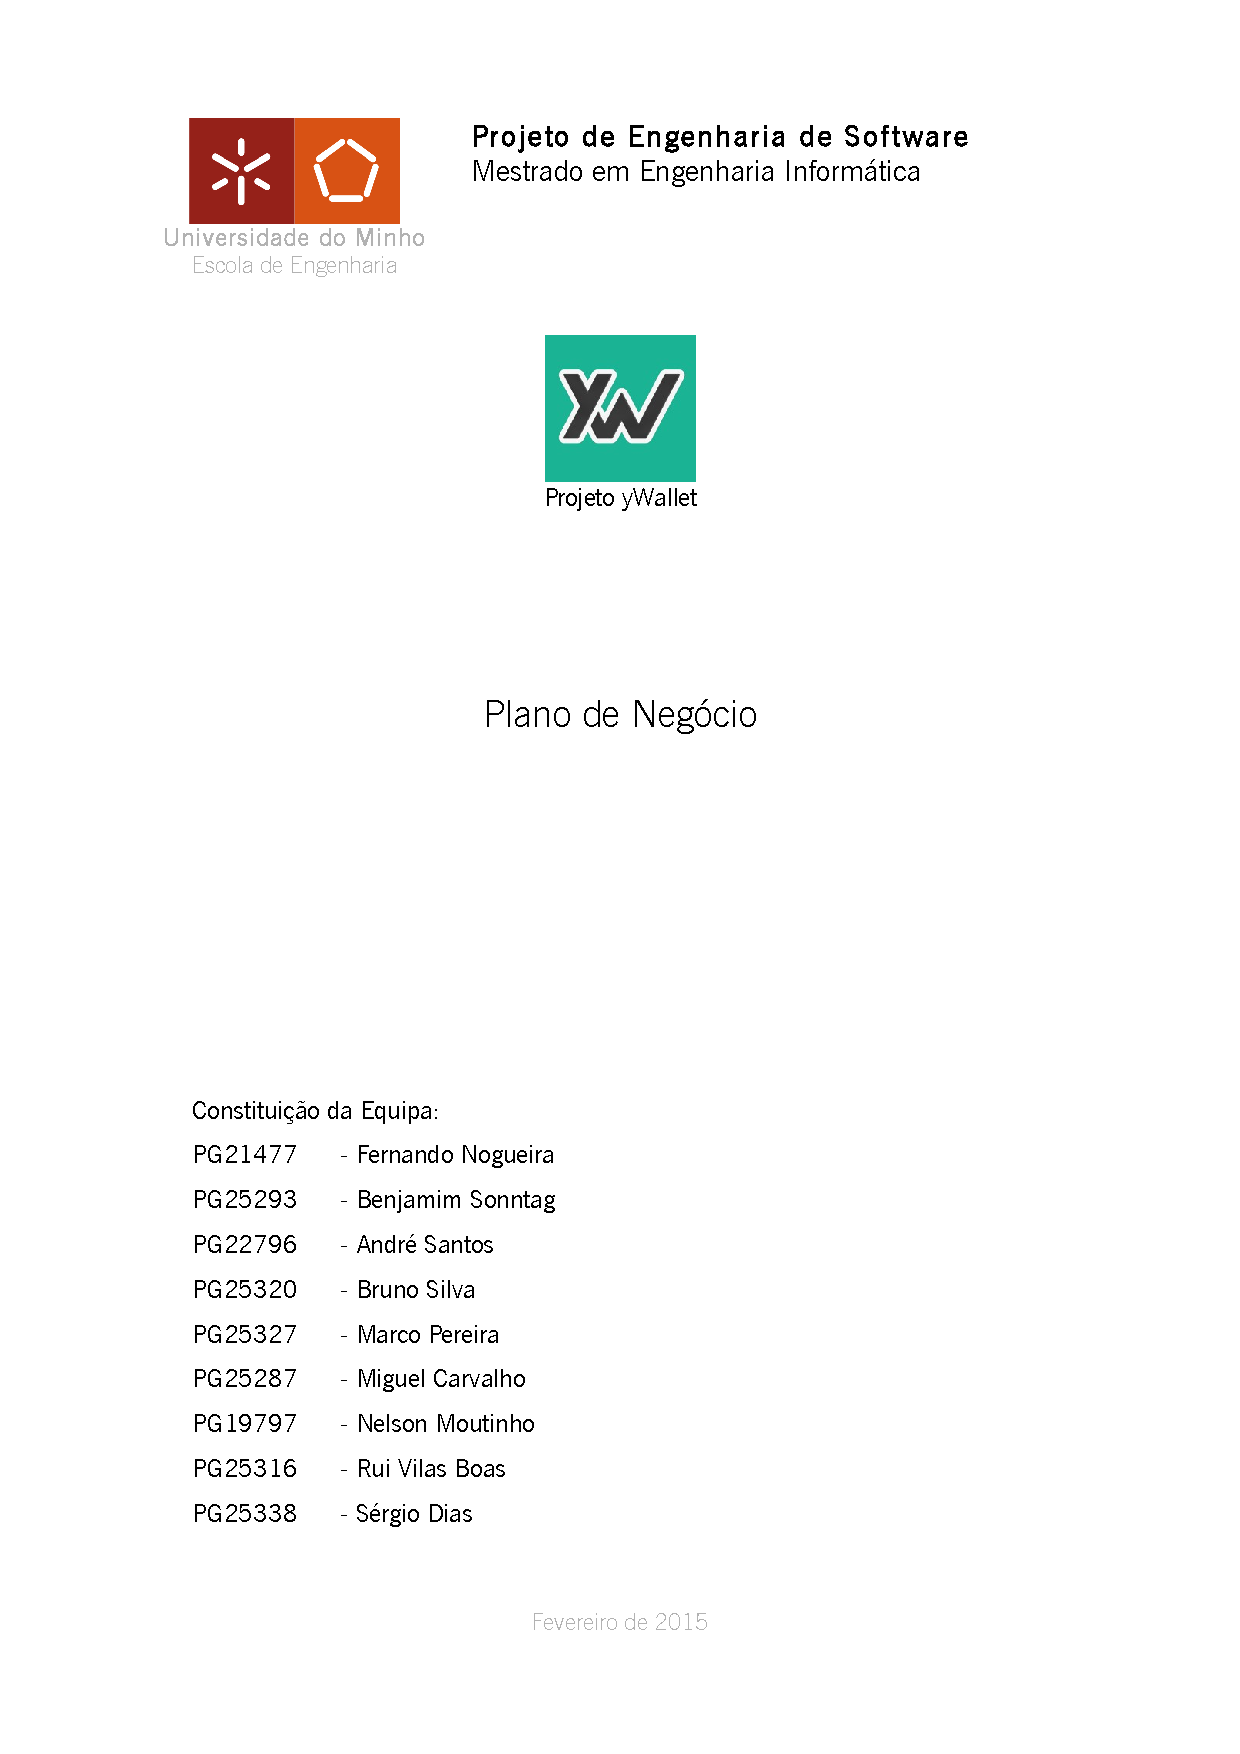
\includepdf[pages=-]{capa}

\tableofcontents

\listoftables

\newpage
\section{Sumário Executivo}
\label{sec:sumario_executivo}

\subsection{Objectivo do Projecto}
\label{subsec:objectivo_do_projecto}

O yWallet é um sistema de gestão pessoal de dinheiro. É orientado para as crianças e os seus pais, e tem funcionalidades de controlo parental e de pagamentos móveis via carteiras digitais.

\subsection{Missão do Projecto}
\label{subsec:missao_do_projecto}

O principal propósito do yWallet é permitir às crianças gerir o dinheiro que os pais, entre outros, lhes fornecem, auxiliando-os através de relatórios de utilização e limites sobre a sua utilização, entre outras funcionalidades. Além disto, permite aos seus pais monitorizar e controlar a utilização que os filhos fazem do seu dinheiro. Assim será possível contribuir com sucesso para a educação financeira das crianças.

\subsection{Mercado Potencial}
\label{subsec:mercado_potencial}

O mercado potencial do yWallet é o mercado internacional, pois o nosso produto não se limita em nenhum aspecto que tornasse apenas viável a sua utilização em determinadas zonas geográficas, e a necessidade que satisfaz é universal. Portanto, quaisquer pessoas com filhos que desejam educar os seus filhos financeiramente são potenciais clientes.

\subsection{Características Inovadoras e/ou Diferenciadoras do Serviço}
\label{subsec:caracteristicas_inovadoras_e/ou_Diferenciadoras_do_Servico}

Existem várias soluções com um âmbito semelhante a do yWallet, no entanto não existe uma que execute bem a componente de controlo parental e permita também o controlo pessoal por parte da criança, e além disto integre sistemas de pagamento através de carteiras digitais.

\subsection{Montante Investido e Lucros}
\label{subsec:montante_investido_e_lucros}

Como é típico num projecto iniciado num contexto académico, não houve custos iniciais quer de salários para a equipa do projecto, quer de arrendamento de instalações, nem de equipamento para desenvolvimento.

As tecnologias utilizadas não implicaram custos, visto que são todas gratuitas e os equipamentos necessários foram ou fornecidos pela universidade ou já estavam em posse da equipa do projecto quando este foi iniciado.

Durante o ano de 2015 está previsto um investimento inicial de 34.120,00 euros, onde comtemplam os custos associados com os recursos humanos e de equipamentos, entre outros.
É estimado o projecto tornar-se lucrativo a partir do seu 2º ano de actividade, sendo o lucro acumulado aproximadamente 19.361,77 euros.

\newpage
\section{A Ideia do Projecto}
\label{sec:a_ideia_do_projecto}

Hoje em dia, é tipico qualquer criança fazer compras com alguma regularidade, quer seja em lojas físicas ou virtuais. Uma vez que não possuem uma fonte de rendimento própria, o seu dinheiro é tipicamente proveniente dos seus progenitores ou familiares, quer sobre a forma de mesadas ou semanadas, ou de prendas pontuais.

Com isto surge um problema clássico: as crianças por regra não compreendem o valor do dinheiro, e como tal não o conseguem controlar correctamente. Há então uma necessidade da criança ser educada financeiramente, que por regra os seus progenitores se responsabilizam.

No entanto, o acompanhamento contínuo da criança pode tornar-se difícil, em vários aspectos: no fornecimento regular de dinheiro à criança, nas interrogações constantes às crianças para perceber como estão de facto a usar o seu dinheiro que podem fomentar um ambiente de desconfiança, no estabelecimento de limites, ou simplesmente na contabilidade dos gastos.
É neste contexto que a nossa solução se insere: ela auxilia os pais a fazerem depósitos regulares nas contas dos filhos de forma automática, permite consultar facilmente a qualquer momento o histórico de gastos, permite quer aos filhos quer aos pais estabelecerem limites de utilização, para controlar melhor os gastos, e ainda apela às necessidades das crianças, disponibilizando funcionalidades como objectivos de poupança, para promover a sua educação financeira, aliviando assim os progenitores de parte dessa responsabilidade.

\subsection{Vantagens do Produto}
\label{subsec:vantagens_do_produto}

Como já foi exposto, a utilização deste produto irá facilitar bastante o processo de fornecer dinheiro às crianças e educá-las na sua utilização, tornando estes processos em experiências muito mais agradáveis quer para os pais como para os filhos. Como uma solução integrada quer de gestão de dinheiro como de pagamento, torna-se mais simples de utilizar e muito mais desejável, sendo uma verdadeira alternativa aos concorrentes disponíveis, e uma solução muito superior para clientes que actualmente fazem esta gestão manualmente.

\subsection{Factores de Sucesso}
\label{subsec:factores_de_sucesso}

Com o objecto de ter um produto bem sucedido, há alguns aspectos que se devem ter em conta:

\begin{itemize}
\item O produto deve diminuir o tempo associado a tarefas que os utilizadores executem, auxiliando-os nestas e automatizando-as sempre que possível;
\item O produto deve ser simples de instalar, e ter o menor número possível de limitações tecnológicas nesse aspecto (deve estar disponível num grande número de plataformas, por exemplo);
\item O produto deve ser intuítivo e simples de utilizar, para apelar ao maior número de utilizadores e não os confundir.
\end{itemize}

\newpage
\section{Análise do Mercado}
\label{sec:analise_do_mercado}


\subsection{Segmentação de Clientes}
\label{subsec:segmentacao_de_clientes}

Os possíveis clientes alvo do yWallet são progenitores ou tutores com crianças, adolescentes ou jovens adultos que estejam financeiramente dependentes dos seus progenitores ou tutores, e pretendam utilizar uma solução que lhes permita gerir o dinheiro, e possivelmente auxiliar na educação financeira dos mesmos.

Considerando a natureza do métodos de pagamento (utilizando plataformas móveis), devem ser explorados mercados com o maior potencial possível, pois são os mais viáveis.

Tendo isto em conta, numa primeira fase o serviço estará disponível nos EUA, visto que neste mercado há mais maturidade tecnológica e um maior grau de aceitação de novas tecnologias ou serviços tecnológicos.

Numa segunda fase, após um potencial processo de evolução do produto ao nível das suas funcionalidades e limitações tecnológicas, o produto irá ser lançado globalmente.

\subsection{Estudo Realizado}
\label{subsec:estudo_realizado}

Com o proposito de compreender melhor as necessidades dos nossos potenciais clientes, realizamos questionários e entrevistas através das quais identificamos as funcionalidades mais desejáveis, e os principais problemas a serem resolvidos. São os seguintes:

\begin{itemize}
\item Facilitar o processo de fornecimento de dinheiro aos filhos;
\item Permitir o controlo das despesas, quer através da consulta de um histórico de gastos, quer através do estabelecimento de limites de usos;
\item Não estar limitado na sua utilização (por exemplo, um dos concorrentes apenas gere os gastos feito nas escolas);
\item Permitir interação com outros utilizadores;
\item Permitir aos filhos controlarem o seu próprio uso do dinheiro;
\item Evitar que o controlo por parte dos pais seja demasiado intrusivo;
\item Permitir o estabelecimento de objectivos ou metas de poupança, para justificar e fomentar a boa gestão de dinheiro.
\end{itemize}

Os estudos também nos permitiram identificar o público alvo com maior detalhe (o intervalo de idades com maior interesse são dos 11 aos 18 anos) e justificar o produto, já que revelou grande interesse por parte de todos envolvidos nos questionários e nas entrevistas.

\subsection{Análise da Concorrência}
\label{subsec:analise_da_concorrência}

A concorrência também foi analisada (os detalhes podem ser vistos no documento anexo “Visão do Produto e Documento de Requisitos”). Desta análise resultou um conjunto de aspectos que a nossa solução deve suportar, para satisfazer os clientes. Estes aspectos são os seguintes:

\begin{itemize}
\item Permitir controlo das despesas;
\item Não estar limitado a certos contextos (por exemplo, contexto de uma escola);
\item Ter funcionalidades relacionadas com poupanças;
\item Evitar comissões nos processos de transferência de dinheiro;
\item Suportar notificações em certas condições;
\item Automatizar o processo de fornecimento de dinheiro aos filhos;
\item Permitir transferências entre utilizadores;
\item Suportar pagamentos através de dispositivos móveis, com recurso a várias tecnologias.
\end{itemize}

\subsection{Fornecedores e Parcerias}
\label{subsec:fornecedores_e_parcerias}

Para tornar possível este projecto, foram necessários vários recursos que felizmente foram disponibilizados por várias entidades.

A Universidade do Minho forneceu-nos um espaço que utilizamos para as nossas reuniões semanais, onde discutimos e definimos o projecto, e onde também o desenvolvemos.

A solução em si não seria possível sem a integração do sistema CoinBase, que faz a gestão do dinheiro dos utilizadores e nos permite fazer transacções com outras entidades.

\newpage
\section{Estratégia de Negócio}
\label{sec:estrategia_de_negocio}

\subsection{Marketing Mix}
\label{subsec:marketing_mix}

O Marketing Mix é uma análise dos principais componentes de uma estratégia de marketing. As quatro componentes que são exploradas com esta análise são o produto, o preço, o ponto de venda/distribuição e a promoção.

\subsubsection{Produto}
\label{subsubsec:produto}

O produto em si já foi apresentado ao longo deste documento e nos documentos anexos.

\subsubsection{Preço}
\label{subsubsec:preco}

Considerando que o nosso produto vai ter de conquistar clientes novos, alguns dos quais são neste momento clientes de outros produtos, decidimos investir numa estratégia adequada:

\begin{itemize}
\item No primeiro ano de operação, existirá apenas um perfil grátis de utilização, para promover o produto;
\item Nos anos seguintes, haverão dois perfis de utilizadores: um grátis de funcionalidades reduzidas, e outro pago com funcionalidades acrescidas, que inclui dashboards mais detalhadas, utilizar regras de limites e notificações customizáveis, e a possibilidade de associar mais do que um filho à sua conta. Esta versão paga terá um custo de \$10 por mês.
\end{itemize}

\subsubsection{Ponto de Venda/Distribuição}
\label{subsubsec:ponto_de_venda/distribuicao}

Como o nosso produto é uma plataforma web, está imediatamente acessível no endereço www.ywallet.co.

\subsubsection{Promoção}
\label{subsubsec:promocao}

Para promover o nosso produto, iremos utilizar os social media para fazer uma campanha promocional, e também iremos recompensar os primeiros clientes com benefícios exclusivos, especialmente se estes convidarem os seus amigos para serem novos clientes da plataforma.


\newpage
\section{Planeamento Operacional}
\label{sec:planeamento_operacional}


\subsection{Suporte de Utilização}
\label{subsec:suporte_de_utilizacao}

Para auxiliar eventuais clientes que tenham dúvidas ou apresentem problemas na utilização do yWallet, existirá um serviço de helpdesk que esclarecerá quaisquer dúvidas que se apresentem.


\subsection{Plano de Acções}
\label{subsec:plano_de_accoes}

O plano de acções é apresentado em detalhe no documento anexo “Plano do Projecto”.

\newpage
\section{Projeções Financeiras}
\label{sec:projecoes_financeiras}

Para justificar os investimentos e preparar o futuro, é necessário fazer projeções financeiras, sendo possível assim atestar a viabilidade do projecto.

\subsection{Projeções de Vendas}
\label{subsec:projecoes_de_vendas}

Como foi anteriormente referido, o mercado inicial onde pretendemos lançar o nosso produto é nos Estados Unidos da América. Segundo um estudo recente \cite{POP1}, o número de crianças nos EUA na faixa etária dos 12-17 será aproximadamente 22.7 milhões. 
Desta população, apenas parte verifica as condições necessárias e estaria interessada no yWallet. Com isto em conta, projectamos o seguinte volume de negócio:

\begin{table}[h]
\centering
\begin{tabular}{|c|c|c|c|c|}
\hline
\textbf{Ano}            & 2015   & 2016         & 2017         & 2018         \\ \hline
\textbf{Subscrições Vendidas (unid.)} & 500    & 1000         & 2000         & 5000         \\ \hline
\textbf{Taxa de Crescimento (\%)}     & -      & 200\%        & 250\%        & 500\%        \\ \hline
\textbf{Preço unitário (\$)}          & -      & 10\EUR/mês      & 10\EUR/mês      & 10\EUR/mês      \\ \hline
\textbf{Total (\$)}                   & \$0,00 & \$120.000,00 & \$240.000,00 & \$600.000,00 \\ \hline
\end{tabular}
  \caption{Volume de Negócio}
\end{table}

\subsection{Fornecimentos e Serviços Externos}
\label{subsec:fornecimentos_e_servicos_externos}

Para o funcionamento regular da empresa estão inerentemente associados custos.

Estes custos englobam serviços essenciais, como o aluguer de um espaço de trabalho, dos serviços de electricidade, água, comunicações, entre outros. A tabela seguinte contém a previsão destes gastos no primeiro ano de operação.


\begin{table}[h]
\centering
\begin{tabular}{|c|c|c|}
\hline
                               & \textbf{Valores Mensais (\EUR)} & \textbf{Total Anual (\EUR)} \\ \hline
\textbf{Servidores e Domínio}   & 40                           & 480                      \\ \hline
\textbf{Renda}                  & 150                          & 1.800                    \\ \hline
\textbf{Água, Luz e Limpeza}    & 60                           & 720                      \\ \hline
\textbf{Material de Escritório} & 25                           & 300                      \\ \hline
\textbf{Comunicações}           & 50                           & 600                      \\ \hline
\textbf{Deslocações}            & 60                           & 720                      \\ \hline
\textbf{Total}                  & 385                          & 4.620                    \\ \hline
\end{tabular}
  \caption{Fornecimentos e Serviços Externos}
\end{table}

\pagebreak
\subsection{Custo com o Pessoal}
\label{subsec:custo_com_o_pessoal}

Numa fase inicial, será necessário completar o produto até ele se encontrar num estado completamente funcional, e quando se encontrar funcional, começar a gerir os novos clientes.

Uma vez que o desenvolvimento do produto está quase terminado, e o número inicial de clientes será diminuto, considera-se que no primeiro ano de operação serão suficientes 3 colaboradores. Nos anos consequentes, este número aumenta para 5 colaboradores em 2016 e 10 colaboradores em 2017, pois nesse ponto a empresa estará mais desenvolvida e começará a extender o seu âmbito para novos mercados.

\begin{table}[h]
\centering
\begin{tabular}{|c|c|c|c|}
\hline
                                 & \textbf{2015} & \textbf{2016} & \textbf{2017} \\ \hline
\textbf{Vencimentos (\EUR)}             & 25.000        & 42.000        & 84.000        \\ \hline
\textbf{Encargos (\EUR)}                & 2.000         & 2.000         & 2.000         \\ \hline
\textbf{Subsídio de Alimentação (\EUR)} & 2.500         & 4.200         & 8.400         \\ \hline
\textbf{Total (\EUR)}                   & 29.500        & 48.200        & 94.400        \\ \hline
\end{tabular}
  \caption{Custos com o Pessoal}
\end{table}

\subsection{Fluxo de Caixa}
\label{subsec:fluxo_de_caixa}

As projecções financeiras permitem-nos planear o balanço entre as receitas e os gastos ao longo do tempo. Focando-nos nos objectivos em longo prazo, convém fazer um planeamento que tenha em consideração estes aspectos, para identificar a viabilidade do projecto. Assim, considerando as receitas e os gastos nos primeiros anos de operação, como podemos ver pela tabela seguinte, projecta-se que se compensa o investimento inicial e começa-se a fazer lucro a partir do segundo ano, 2016.

\begin{table}[h]
\centering
\begin{tabular}{|c|c|c|c|}
\hline
                                                       & \textbf{2015} & \textbf{2016} & \textbf{2017} \\ \hline
\textbf{Receitas (\EUR)}                                  & 0,00          & 106.335,89    & 212.671,78    \\ \hline
\textbf{Despesas Fornecimentos e Serviços Externos (\EUR)} & 4.620,00      & 4.620,00      & 4.620,00      \\ \hline
\textbf{Custos Pessoal (\EUR)}                            & 29.500,00     & 48.200,00     & 94.400,00     \\ \hline
\textbf{Lucro Anual (\EUR)}                               & -34.120,00    & 53.515,89     & 113.651,78    \\ \hline
\textbf{Lucro Acumulado (\EUR)}                           & -34.120,00    & 19.361,77     & 133.013,55    \\ \hline
\end{tabular}
  \caption{Fluxo de Caixa}
\end{table}

\newpage
\section{Bibliografia}
\label{sec:bibliografia}

\begin{thebibliography}{9}

\bibitem{POP1}
  \emph{POP1 CHILD POPULATION: NUMBER OF CHILDREN (IN MILLIONS) AGES 0–17 IN THE UNITED STATES BY AGE, 1950–2013 AND PROJECTED 2014–2050}, 2014.
  Disponível em:
  <http://www.childstats.gov/americaschildren/tables/pop1.asp>.
  [01 Fevereiro 2015]

\end{thebibliography}

\end{document}